\documentclass{article}
\usepackage[utf8]{inputenc}

\title{Exam 2}
\author{Benny Chen}
\date{\today}

\usepackage{color}
\usepackage{amsthm}
\usepackage{amssymb} 
\usepackage{amsmath}
\usepackage{listings}
\usepackage{xcolor}
\usepackage{listings}
\usepackage{graphicx}
\usepackage[hidelinks]{hyperref}

\definecolor{codegreen}{rgb}{0,0.6,0}
\definecolor{codegray}{rgb}{0.5,0.5,0.5}
\definecolor{codepurple}{rgb}{0.58,0,0.82}
\definecolor{backcolour}{rgb}{0.95,0.95,0.92}

\lstdefinestyle{mystyle}{
    backgroundcolor=\color{backcolour},   
    commentstyle=\color{codegreen},
    keywordstyle=\color{magenta},
    numberstyle=\tiny\color{codegray},
    stringstyle=\color{codepurple},
    basicstyle=\ttfamily\footnotesize,
    breakatwhitespace=false,         
    breaklines=true,                 
    captionpos=b,                    
    keepspaces=true,                 
    numbers=left,                    
    numbersep=5pt,                  
    showspaces=false,                
    showstringspaces=false,
    showtabs=false,                  
    tabsize=2
}

\lstset{style=mystyle}

\begin{document}

\maketitle

\section{True or False plus explanation}

\begin{enumerate}
    \item In the soft-margin linear support vector machine classification problem (the one with the slack variables), it is not possible to control the relative importance of maximizing the margin and minimizing the error.
    \item In soft-margin SVM, suppose slack variable $\epsilon_i = 0.2$ for some $i$. Then the corresponding
    datapoint $x_i$ for this slack variable is a support vector since it is classified incorrectly.
\end{enumerate}

\subsection*{Solutions}

\begin{enumerate}
    \item False. The relative importance of maximizing the margin and minimizing the error can be controlled by $C$. A large $C$ will result in a small margin and a small $C$ will result in a large margin.
    \item False. The datapoint $x_i$ is not a support vector since it is classified correctly. This is because the slack variable $\epsilon_i$ is greater than 0 and less than 1. If $\epsilon_i$ was equal to 1, then $x_i$ would be a support vector.
\end{enumerate}

\newpage

\section{K-Means Clustering}

Consider the 4 data points shown in the following figure. The distance between each data point to the centroid C is R.
\begin{center}
    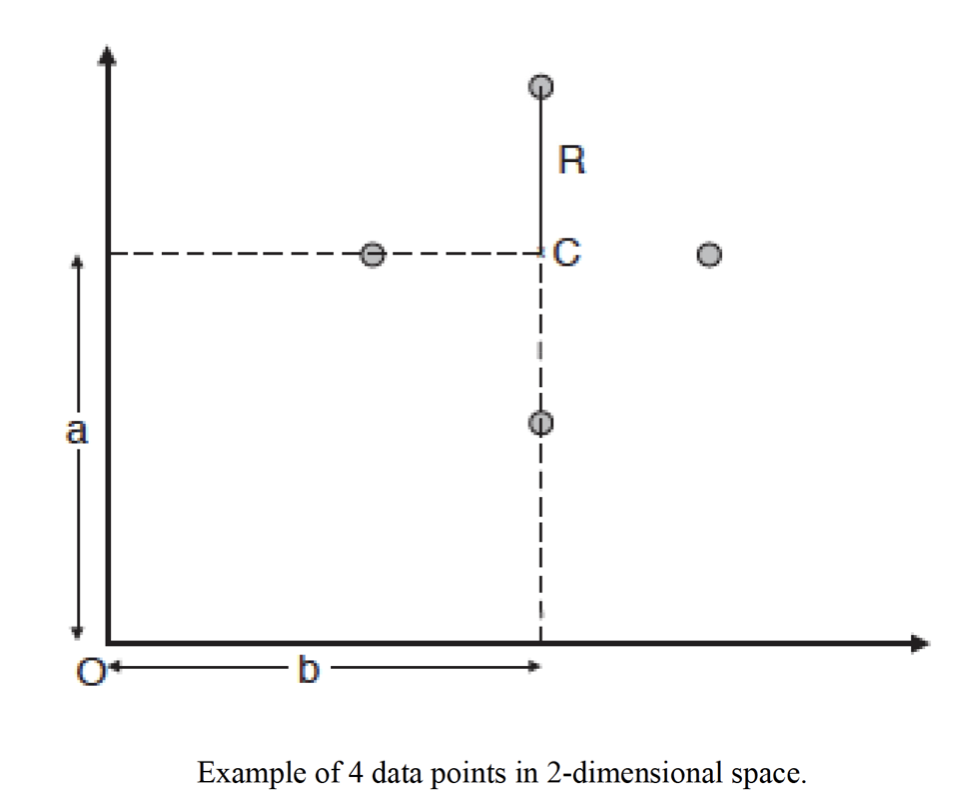
\includegraphics[scale=0.5]{./images/Q2AB.png}
\end{center}

\begin{enumerate}
    \item Compute the total SSE of the data points to the centroid, C.
    \item Compute the total SSE of the data points to the origin, O.
    \item Using parts (a) and (b), compute the SSE for the 8 data points shown below with respect to the centroid, D. Note that points each group (cluster) of data points lie on a circle of radius R/2. Also, the figure is symmetric with respect to the horizontal line running through D.
\end{enumerate}
\begin{center}
    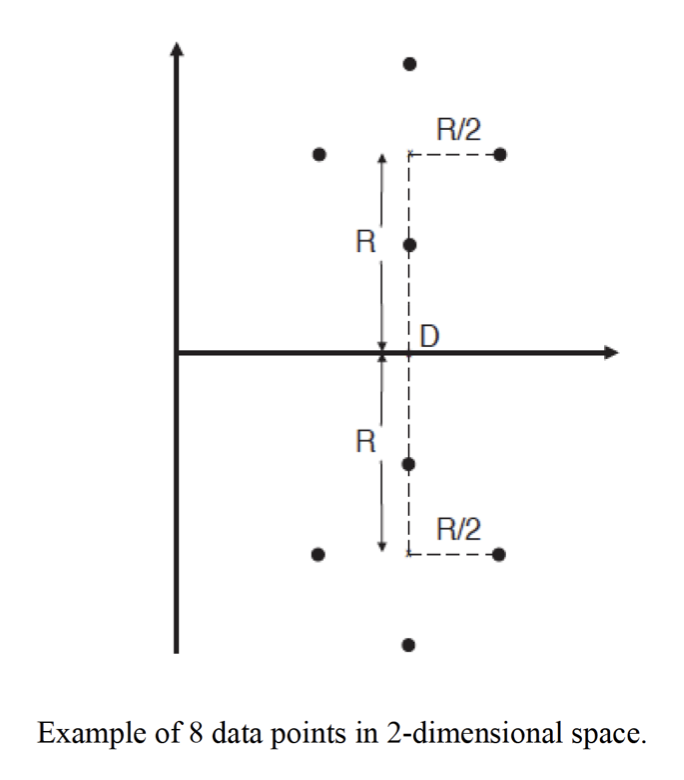
\includegraphics[scale=0.5]{./images/Q2C.png}
\end{center}

\subsection*{Solutions}

\begin{equation}
    SSE = \sum_{i=1}^{K} \sum_{x \in C_i}^{} dist^2(m_i, x)
\end{equation}

\begin{enumerate}
    \item 
    \begin{equation}
        SSE = R^2 + R^2 + R^2 + R^2 = 4R^2
    \end{equation}
    \item 
    \begin{equation}
            dist^2(O, R_1) = {(b-R)}^2 + {(a)}^2
    \end{equation}
    \begin{equation}
            dist^2(O, R_2) = {(b)}^2 + {(a-R)}^2
    \end{equation}
    \begin{equation}
            dist^2(O, R_3) = {(b+R)}^2 + {(a)}^2
    \end{equation}
    \begin{equation}
            dist^2(O, R_4) = {(b)}^2 + {(a+R)}^2
    \end{equation}
    \begin{equation}
        SSE = {(b-R)}^2 + {(a)}^2 + {(b)}^2 + {(a-R)}^2 + {(b+R)}^2 + {(a)}^2 + {(b)}^2 + {(a+R)}^2
    \end{equation}
    \begin{equation}
        SSE = 4a^2 + 4b^2 + 4R^2
    \end{equation}
    \item 
    \begin{equation}
        dist^2(D, R_1) = {(\frac{R}{2})}^2
    \end{equation}
    \begin{equation}
        dist^2(D, R_2) = {(\frac{3R}{2})}^2
    \end{equation}
    \begin{equation}
        dist^2(D, R_3) = {(R)}^2 + {(\frac{R}{2})}^2
    \end{equation}
    \begin{equation}
        dist^2(D, R_4) = {(R)}^2 + {(\frac{R}{2})}^2
    \end{equation}
    \begin{equation}
        SSE = {(\frac{R}{2})}^2 + {(\frac{3R}{2})}^2 + {(R)}^2 + {(\frac{R}{2})}^2 + {(R)}^2 + {(\frac{R}{2})}^2
    \end{equation}
    \begin{equation}
        SSE = 5R^2
    \end{equation}
    Since the figure is symmetric with respect to the horizontal line running through D, the SSE for the 8 data points is $5R^2 + 5R^2 = 10R^2$.
\end{enumerate}

\end{document}